
\documentclass[11pt,a4paper,twocolumn]{article}
\usepackage{amsmath}
\usepackage{amsfonts}
\usepackage{amssymb}
\usepackage{graphicx}
\usepackage[utf8]{inputenc}
\usepackage{textcomp} 
\usepackage{ngerman}
\usepackage{listings}
\usepackage[american,ngerman]{babel}

\lstset{literate=%
    {Ö}{{\"O}}1
    {Ä}{{\"A}}1
    {Ü}{{\"U}}1
    {ß}{{\ss}}1
    {ü}{{\"u}}1
    {ä}{{\"a}}1
    {ö}{{\"o}}1
    {~}{{\textasciitilde}}1
}

\lstset{
  basicstyle=\scriptsize,
  tabsize=2
}

\title{Phoenixtool Server API Dokumentation}
\author{Roberts Kolosovs}

\begin{document}
\maketitle

\section*{Einleitung}
Dieses Dokument beschreibt die Schnittstelle des Phönixtool-Servers. Der Informationsaustausch mit dem Server erfolgt im JSON-Format \footnote{http://www.json.org/}.\\
Abschnitt \ref{s:data_read} beschreibt die Repräsentation des Spielstandes und dessen Auslesen. Im Abschnitt \ref{s:data_write} erklären wir, wie man einen neuen Spielstand auf den Server schreibt. Der Abschnitt \ref{s:security} beschreibt unser Sicherheitskonzept und den Login-View. Die Struktur unserer Spielzüge ist beschrieben im Abschnitt \ref{s:turnstructure}. Die darin verwendeten Events werden einzeln im Abschnitt \ref{s:events} beschreiben.

\section{Lesen von Spieldaten}\label{s:data_read}
In diesem Abschnitt beschreiben wir unsere Repräsentation des Spielstandes und den Format, in dem es vom Server geliefert wird. Die Liste der Reiche ist im Unterabschnitt \ref{ss:read_realms} beschreiben. Der Unterabschnitt \ref{ss:read_armies} beschreibt das Format, in dem Armeen und Flotten geliefert werden. Die Gebäude sind im Unterabschnitt \ref{ss:read_buildings}. Die Geländetypen des Spielfelds sind in \ref{ss:read_field} und die Flüsse sind in \ref{ss:read_rivers} beschrieben. Zu Letzt sind die Gebiete der Reiche in \ref{ss:read_borders} beschreiben.
\subsection{Reiche}\label{ss:read_realms}
Die Liste der am Spiel teilnehmenden (oder in der Vergangenheit teilgenommenen) Reiche erhält man mit einer Anfrage an "/databaseLink/getrealms/". Die Antwort kommt in folgender Form:
\begin{lstlisting}
[{
  'active': True für im Spiel aktive Reiche,
  'color': Reichsfarbe als "r,g,b",
  'name': Voller Reichsname,
  'homeTurf': Heimatgelände (0 - 8),
  'tag': Reichskürzel (3 Zeichen)
}, ...]
\end{lstlisting}
Die Reihenfolge der Reiche im Array sollte deren Reihenfolge in der DB entsprechen. Das Reich mit dem DB-Key n sollte also im Array an der Stelle n-1 stehen. Die Reiche sollten aus der Datenbank nicht gelöscht werden sonder auf inaktiv gesetzt werden.\\
Das Feld 'active' wird auf False gesetzt falls das Reich gänzlich aus dem Spiel ausscheidet und nur für historische Nachvollziehbarkeit in der Datenbank gelistet wird. Wird das Reich nur umbenannt, an andere Spieler übergeben, ändert seine Farbe oder ähnliches, so soll der Datenbankeintrag stattdessen lieber modifiziert werden.\\
Die Reichsfarbe, in welcher das Reich auf der Karte dargestellt werden sollte wird als ein String im 'color'-Feld gespeichert. Der String ist genau 11 Zeichen lang und enthält die RGB-Werte der Farbe im Dezimalformat (000 - 255) durch Komata ohne Leerzeichen getrennt. Schwarz wäre also als "000,000,000" während "255,000,000" rot und "090,090,090" ein Grauton wäre.\\
Im Feld 'homeTurf' wird das Typ des Heimatgeländes eines Reiches (in der Regel der Feldtyp, auf dem die Hauptstadt steht) angegeben. Die Nummerierung der Feldtypen wird in \ref{ss:read_field} beschrieben.\\
Das 'tag'-Feld gibt ein Reichskürzel aus genau 3 Zeichen an. Dieses ist als eine Möglichkeit Reiche zu identifizieren gedacht, die kürzer und beständiger als der volle Name und gleichzeitig menschenlesbarer als der Datenbank-Key ist.
\subsection{Armeen}\label{ss:read_armies}
Die Heere (Armeen) und Flotten erhält man mit einer Anfrage an "/databaseLink/armydata/". Die Anfrage muss wie folgt aussehen:
\begin{lstlisting}
{'authorization': Auth-Token}
\end{lstlisting}
Das Authentifizierungs-Token identifiziert einen eingeloggten Nutzer und ist in \ref{s:security} beschrieben. Die Antwort hat das folgende Format:
\begin{lstlisting}
[{
  'realm': Kontrolierendes Reich (Kürzel),
  'armyId': Armeenummer (Phoenix),
  'count': Truppen-/Schiffsanzahl,
  'leaders': Heerführeranzahl,
  'mounts': mitgeführte Reittiere,
  'lkp': leichte Katapulte/Kriegsschiffe,
  'skp': schwere Katapulte/Kriegsschiffe,
  'x': x-Koordinate der Position,
  'y': y-Koordinate der Position,
  'isGuard': True für Gardeheere/ -flotten,
  'isLoadedIn': Armeenummer der 
                transportierenden Flotte,
  'movementPoints': Bewegungspunkte 
					der Armee,
  'heightPoints': Höhenpunkte der Armee
}]
\end{lstlisting}
Fußheere, Reiterheere und Flotten werden Serverseitig gleich gespeichert. Welches gemeint ist und somit, welche Bedeutung die einzelnen Felder haben, lässt sich aus dem 'armyId'-Feld ablesen. Die Fußheere haben Nummern 101-199, Reiterheere 201-299 und Flotten 301-399.\\
Je nach dem, als welchen Nutzer der Authentifizierungs-Token einen identifiziert, bekommt man verschiedene Informationen. Ein Spielleitungs-Nutzer bekommt die richtigen Anzahlen von allen Armeen/Flotten. Ein eingeloggter Spieler bekommt richtige Zahlen für alle Armeen seines Reiches. Für fremde Armeen wird 'isGuard' auf False gesetzt. Die Felder 'count', 'leaders', 'mounts', 'lkp' und 'skp' werden auf -1 gesetzt, was sonst ein ungültiger Wert ist. Für sonstige Nutzer, auch nicht eingeloggte, werden alle Armeen auf diese Art maskiert.
\subsection{Gebäude}\label{ss:read_buildings}
Rüstorte und andere Gebäude werden mit einer Anfrage an "/databaseLink/buildingdata/". Die Antwort kommt in folgender Form:
\begin{lstlisting}
[{
  'realm': Kontrolierendes Reich (Kürzel),
  'name': benutzerdefinierter Name,
  'type': 0 - 8,
  'x': x-Koordinate (außer Straße),
  'y': y-Koordinate (außer Straße),
  'direction': "nw"/"ne"/"e"/"se"/"sw"/"w",
  'firstX': x-Koordinate Straßenanfang,
  'firstY': y-Koordinate Straßenanfang,
  'secondX': x-Koordinate Straßenende,
  'secondY': y-Koordinate Straßenende
}, ...]
\end{lstlisting}
Das 'realm'-Feld ist redundant, da der Besitzer eines Rüstortes mit dem Besitzer des Feldes identisch ist. In der Zukunft sollte es entweder entfernt oder durch den Reichskürzel ersetzt werden. Der benutzerdefinierte Name ist rein kosmetisch und wird nur benutzt, falls einzelne Rüstorte besondere Namen haben sollen. Dies sollte \emph{nicht} benutzt werden, um einzelnen Rüstorten besondere Funktion zu verleihen. Dazu sollten eigene Felder oder Datenbanktabellen angelegt werden. Die Typen sind von 0 bis 8 wie folgt durchnummeriert:
\begin{itemize}
	\item 0. Burg
	\item 1. Stadt
	\item 2. Festung
	\item 3. Hauptstadt
	\item 4. Festungshauptstadt
	\item 5. Mauer
	\item 6. Kaianlage
	\item 7. Brücke
	\item 8. Straße
\end{itemize} 
Alle Gebäude außer Straßen haben "null" als Werte für die Felder 'firstX', 'firstY', 'secondX' und 'secondY'. Ihre Position wird durch die Felder 'x' und 'y' angegeben. Straßen haben "null" als Wert der Felder 'x' und 'y' und werden zwischen den Feldern ('firstX', 'firstY') und ('secondX', 'secondY') gezogen.\\
Mauern, Anlegestellen und Brücken haben im Feld 'direction' eine Richtung, in die sie von ihrem Feld aus zeigen. Die Richtung ist angegeben als Ein- oder Zwei-Buchstaben Kürzel der Himmelsrichtung, wo die Spitzen der Hex-Felder nach Norden und Süden zeigen. Die x-Werte des Koordinatensystems erhöhen sich von Norden nach Süden. Die y-Werte erhöhen sich von Westen nach Osten. Für andere Gebäudetypen ist dieser Wert "null", da es entweder irrelevant ist (Burg, Stadt, Festung, (Festungs)hauptstadt) oder durch ihre mit zwei Koordinatenpaaren angegebene Position gegeben ist (Straße).
\subsection{Spielfeld}\label{ss:read_field}
Die Geländetypen erhält man mit einer Anfrage an "/databaseLink/fielddata/". Die Antwort sieht wie folgt aus:
\begin{lstlisting}
[{
  'type': 0 - 8,
  'x': x-Koordinate,
  'y': y-Koordinate
}, ...]
\end{lstlisting}
Die Typen sind von 0 bis 8 wie folgt durchnummeriert:
\begin{itemize}
	\item 0. See
	\item 1. Tiefsee
	\item 2. Tiefland
	\item 3. Tieflandwald
	\item 4. Hochland
	\item 5. Bergland
	\item 6. Gebirge
	\item 7. Tieflandwüste
	\item 8. Tieflandsumpf
\end{itemize}
Andere Werte können benutzt werden, um undefinierte Felder zu beschreiben: Das Feld existiert, hat aber noch keinen Geländetyp zugewiesen.\\
Das Koordinatensystem hat ihren Ursprung in der Mitte der Karte. Das obere linke Quadrant hat negative x- und y-Werte. Das obere rechte Quadrant hat positive x- und negative y-Werte. Das untere rechte Quadrant hat positive x- und y-Werte und das untere linke Quadrant hat negative x- und positive y-Werte.\\
Die Zeilen mit ungeraden y-Werten sind den Zeilen mit geraden y-Werten gegenüber um ein halbes Feld nach links verschoben. Da es sich um Hex-Felder handelt, ergeben sich die Nachbarschaftsverhältnisse in den Abbildungen \ref{fig:neighboring_even} und \ref{fig:neighboring_odd}.
\begin{figure}[!ht]
\centering
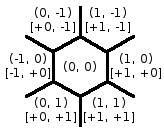
\includegraphics{neighboring_even}
\caption{Nachbarschaft geradzahlige Zeilen}
\label{fig:neighboring_even}
\end{figure}
\begin{figure}[!ht]
\centering
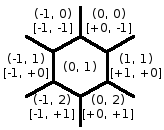
\includegraphics{neighboring_odd}
\caption{Nachbarschaft ungeradzahlige Zeilen}
\label{fig:neighboring_odd}
\end{figure}
\subsection{Flüsse}\label{ss:read_rivers}
Um die Flüsse zu erhalten, muss man eine Anfrage an "/databaseLink/getriverdata/" schicken. Die Antwort kommt in folgender Form:
\begin{lstlisting}
[{
  'firstX': x-Koordinate 1. Feld,
  'firstY': y-Koordinate 1. Feld,
  'secondX': x-Koordinate 2. Feld,
  'secondY': y-Koordinate 2. Feld
}, ...]
\end{lstlisting}
Da Flüsse immer auf den Kanten zwischen zwei Feldern sind, werden sie durch die x- und y-Koordinaten dieser zwei Felder beschreiben.
\subsection{Grenzen}\label{ss:read_borders}
Die Reichsgebiete erhält man durch eine Anfrage an "/databaseLink/getborderdata/". Das Antwortformat ist wie folgt:
\begin{lstlisting}
[{
  'tag': Kontrolierendes Reich (Kürzel),
  'land': [
    [x-Koordinate, y-Koordinate], ...
  ]
}, ...]
\end{lstlisting}
Die Reichsgrenzen sind als Arrays von Feldern angegeben, wobei jedes Feld ein Array von zwei Koordinaten ist. Die Felder sind nach Reichen sortiert. Das heißt, das Array der Reichsgrenzen enthält ein Objekt für jedes aktive Reich. Diese Objekte enthalten die Felder 'tag', welches den drei-Buchstaben-Kürzel des Reiches enthält, und 'land', welches das oben beschriebene Array von Feldern enthält.

\section{Schreiben von Spieldaten}\label{s:data_write}
Dieser Abschnitt beschreibt, mit welchen Anfragen und in welchem Format die Änderungen an dem Spielstand auf den Server geschrieben werden können. Analog zum Abschnitt \ref{s:data_read} beschreiben die Unterabschnitte \ref{ss:write_armies}, \ref{ss:write_buildings}, \ref{ss:write_fields}, \ref{ss:write_rivers} und \ref{ss:write_borders} die Formate für Armeen/Flotten, Gebäude, Geländetypen, Flüsse und Reichsgebiete.
\subsection{Armeen}\label{ss:write_armies}
Man speichert die Armeen in dem man eine Anfrage an "/databaseLink/savearmydata/" schickt. Die Anfrage muss wie folgt aussehen:
\begin{lstlisting}
{
  'armies': [
    'armyId': Armeenummer (Phoenix),
	'count': Truppen-/Schiffsanzahl,
    'leaders': Heerführerzahl,
    'lkp': leichte Katapulte/Kriegsschiffe,
    'skp': schwere Katapulte/Kriegsschiffe,
    'mounts': mitgeführte Reittiere,
    'owner': Kontrolierendes Reich 
               (Kürzel),
    'movementPoints': Bewegungspunkte 
                      der Armee,
    'heightPoints': Höhenpunkte 
                    der Armee,
    'isLoadedIn': True für Landheere 
                  auf Schiffen
  ],
  'authorization': Auth-Token
}
\end{lstlisting}
Das Feld 'armies' enthält die zu schreibenden Armeen als ein Array, das mit dem Stringify-Verfahren zu einem String verpackt wurde. Soll eine Armee gelöscht werden, lässt man sie einfach aus der Liste raus. In diesem Fall wird die Armee serverseitig nicht aus der DB entfernt, aber als 'inactive' markiert. So markierte Armeen sind effektiv gelöscht: Sie werden nicht mit den restlichen Armeen an den Client geschickt und werden nur zur Spielhistorie in der DB behalten. Das 'authorization'-Feld enthält den Authentifizierungs-Token. Nur wenn dieser den User als einen Spielleiter identifiziert, wird diese Anfrage akzeptiert.\\
Die Anfrage liefert Statuscodes mit folgender Bedeutung zurück:
\begin{itemize}
\item 200: Erfolg
\item 401: Nutzer nicht eingeloggt
\item 403: Eingeloggter Nutzer hat keine SL-Rechte
\end{itemize}
\subsection{Gebäude}\label{ss:write_buildings}
Die Gebäude werden mit der Anfrage an "/databaseLink/savebuildingdata/" gespeichert. Der Inhalt der Anfrage muss wie folgt aussehen:
\begin{lstlisting}
{
  'buildings': Gebäude als String,
  'authorization': Auth-Token
}
\end{lstlisting}
Das Feld 'buildings' enthält die zu schreibenden Gebäude als ein String. \textbf{ Nicht maintainable! Dies sollte schnellstmöglich zu einem vernünftigen JSON-Format geändert werden!} Das 'authorization'-Feld enthält den Authentifizierungs-Token. Nur wenn dieser den User als einen Spielleiter identifiziert, wird diese Anfrage akzeptiert.\\
Die Anfrage liefert Statuscodes mit folgender Bedeutung zurück:
\begin{itemize}
\item 200: Erfolg
\item 401: Nutzer nicht eingeloggt
\item 403: Eingeloggter Nutzer hat keine SL-Rechte
\end{itemize}
\subsection{Spielfeld}\label{ss:write_fields}
Die Gebäude werden mit der Anfrage an "/databaseLink/savefielddata/" gespeichert. Der Inhalt der Anfrage muss wie folgt aussehen:
\begin{lstlisting}
{
  'map': Kartenfelder als String,
  'authorization': Auth-Token
}
\end{lstlisting}
Das Feld 'map' enthält die zu schreibenden Felder als ein String. \textbf{ Nicht maintainable! Dies sollte schnellstmöglich zu einem vernünftigen JSON-Format geändert werden!} Das 'authorization'-Feld enthält den Authentifizierungs-Token. Nur wenn dieser den User als einen Spielleiter identifiziert, wird diese Anfrage akzeptiert.\\
Die Anfrage liefert Statuscodes mit folgender Bedeutung zurück:
\begin{itemize}
\item 200: Erfolg
\item 401: Nutzer nicht eingeloggt
\item 403: Eingeloggter Nutzer hat keine SL-Rechte
\end{itemize}
\subsection{Flüsse}\label{ss:write_rivers}
Die Gebäude werden mit der Anfrage an "/databaseLink/saveriverdata/" gespeichert. Der Inhalt der Anfrage muss wie folgt aussehen:
\begin{lstlisting}
{
  'river': Flüsse als String,
  'authorization': Auth-Token
}
\end{lstlisting}
Das Feld 'river' enthält die zu schreibenden Flüsse als ein String. \textbf{ Nicht maintainable! Dies sollte schnellstmöglich zu einem vernünftigen JSON-Format geändert werden!} Das 'authorization'-Feld enthält den Authentifizierungs-Token. Nur wenn dieser den User als einen Spielleiter identifiziert, wird diese Anfrage akzeptiert.\\
Die Anfrage liefert Statuscodes mit folgender Bedeutung zurück:
\begin{itemize}
\item 200: Erfolg
\item 401: Nutzer nicht eingeloggt
\item 403: Eingeloggter Nutzer hat keine SL-Rechte
\end{itemize}
\subsection{Grenzen}\label{ss:write_borders}
Die Gebäude werden mit der Anfrage an "/databaseLink/saveborderdata/" gespeichert. Der Inhalt der Anfrage muss wie folgt aussehen:
\begin{lstlisting}
{
  'borders': [{
    'tag': Kontrolierendes Reich (Kürzel),
    'land': [
      [x-Koordinate, y-Koordinate], ...
    ]   
  }, ... ],
  'authorization': Auth-Token
}
\end{lstlisting}
Das Feld 'borders' enthält die zu schreibenden Grenzen im selben Format wie es vom Server empfangen wurde. Sie müssen mit der Stringify-Methode zu einem String verpackt werden. Das 'authorization'-Feld enthält den Authentifizierungs-Token. Nur wenn dieser den User als einen Spielleiter identifiziert, wird diese Anfrage akzeptiert.\\
Die Anfrage liefert Statuscodes mit folgender Bedeutung zurück:
\begin{itemize}
\item 200: Erfolg
\item 401: Nutzer nicht eingeloggt
\item 403: Eingeloggter Nutzer hat keine SL-Rechte
\end{itemize}

\section{Sicherheit}\label{s:security}
Hier beschreiben wir das Sicherheitskonzept unserer Anwendung und die dazu relevanten Serverinteraktionen. Das generelle Sicherheitsdesign findet man im Unterabschnitt \ref{ss:securityconcept}. Die Login-Interaktion ist beschrieben in \ref{ss:login} und der dabei benutzte CSRF-Token in \ref{ss:csrftoken}. Der Logout ist im Unterabschnitt \ref{ss:logout} erklärt. 
\subsection{Sicherheitsdesign}\label{ss:securityconcept}
Das Phoenixtool setzt alle gängigen Sicherheitsvorkehrungen für Webanwendungen ein, um die Integrität des Spiels sicher zu stellen.\\
Die Kommunikation mit dem Server erfolgt über das HTTPS Protokoll. Ein User muss sich beim Server einloggen um nicht-öffentliche Information zu erhalten und damit seine Anfragen vom Server akzeptiert werden.\\
Der Login erfolgt durch die vom Django-Framework bereitgestellte Infrastruktur und ein eingeloggter User erhält ein Authentifizierungs-Token (authentification token). Dieser muss bei bestimmten Anfragen mitgeschickt werden und der Server überprüft, ob der User für die gegebene Anfrage autorisiert ist. Zum Beispiel ist nur der Spielleiter und der Besitzer einer Armee autorisiert, diese zu bewegen.\\
Um redundante Regelimplementierung zu vermeiden, führt der Server nur die rudimentäre Berechtigungsüberprüfung durch. Die Regeln sind nur in der Client-Anwendung implementiert. Da wir die Integrität der Client-Software nicht sicherstellen können, implementieren wir den Event-Sicherheitsmechanismus. Dieser verhindert, dass ein kompromittierter Spieler-Client die Integrität des gesamten Spieles kompromittiert. Zusätzlich erlaubt es der Spielleitung mehr und feinere Kontrolle über den Spielverlauf.\\
Der Event-Mechanismus verbietet Spielern direkt Änderungen an dem serverseitigen Spielstand zu machen. Stattdessen schreiben sie so genannte "Events" in die Server-Datenbank, welche die Absicht repräsentieren, eine bestimmte Aktion durchzuführen. Diese lädt die Spielleitung dann in ihre Client-Software und transformiert diese dann manuell oder (teil)automatisch in tatsächliche Spielstandänderung.\\
Die Client-Software der Spielleitung ist die selbe Implementierung wie die der Spieler, weshalb immer noch keine redundante Regelimplementierung vorliegt. Die unterschiedlichen Möglichkeiten der Spieler- und SL-Clients beruht ausschließlich auf die unterschiedlichen Authentifizierungstokens und die entsprechende Reaktion des Servers auf die generierte Anfragen. Anderes als bei dem Spieler-Client wird angenommen, dass alle Veränderungen, welche die SL an ihrem Client vornimmt, legitim sind.\\
Die Event-Konstrukte und deren Benutzung sind in den Abschnitten \ref{ss:events_use} und \ref{s:events} beschrieben. 
\subsection{Login}\label{ss:login}
Mit einer Anfrage an "/databaseLink/login/" loggt man sich auf dem Server ein. Die Anfrage muss wie folgt aussehen:
\begin{lstlisting}
{
  'username': Nutzername,
  'password': Passwort
}
\end{lstlisting}
Die Antwort kommt in folgendem Format:
\begin{lstlisting}
{
  'token': Auth-Token,
  'group': 'guest'/'sl'/Reichskürzel
}
\end{lstlisting}
Das 'token'-Feld enthält den Authentifizierungstoken, welchen man braucht, um sich bei anderen Anfragen zu authentifizieren. Das 'group'-Feld enthält einen Text, der beschreibt, als welche Nutzergruppe (bestimmtes Reich, Spielleitung oder Nutzer ohne irgendwelche Rechte) man sich eingeloggt hat. Dies ist nur dazu da, um eine einfach lesbare Bestätigung zu haben, als welcher Nutzer man sich eingeloggt hat. Als fälschungssichere Bestätigung der Nutzeridentität dient das Authentifizierungstoken.\\
\textbf{\emph{Es fehlen mehrere wichtige Sicherheitsmechanismen, die möglichst bald implementiert werden sollen.
\begin{enumerate}
\item Zum Schutz vor Cross Site Request Forgery soll ein CSRF-Token benutzt werden
\item Die Kommunikation mit dem Server soll auf HTTPS umgestellt werden, um man-in-the-middle Angriffe weniger mächtig zu machen
\end{enumerate}}}
\subsection{CSRF Token}\label{ss:csrftoken}
\textbf{\emph{Muss noch implementiert werden.}}
\subsection{Logout}\label{ss:logout}
Um sich auszuloggen muss man eine Anfrage an "/databaseLink/logout/" schicken.

\section{Zugstruktur}\label{s:turnstructure}
In diesem Abschnitt ist erklärt, wie die Zugabfolge des Phönix-Spiels in unserer Software serverseitig umgesetzt ist. Das Auslesen des aktuellen Zuges und die Aktionen, in jedem Zugabschnitt erwartet sind, beschreiben wir in \ref{ss:turn_current}. Wie man den nächsten Zugabschnitt auslöst ist in \ref{ss:turn_next} erklärt. Das System der Events, welche Teil unseres Sicherheitskonzepts sind, werden in der Zugstruktur benutzt. Die Einzelheiten dieser Nutzung sind in \ref{ss:events_use} beschrieben.
\subsection{Aktueller Zug}\label{ss:turn_current}
Die grundsätzliche Zugstruktur jede Runde sieht wie folgt aus:
\begin{itemize}
\item 0. Zug 147. kein Reich
\item 1. Zug 147. Reich 1 Start
\item 1. Zug 147. Reich 1 Ende
\item 2. Zug 147. Reich 2 Start
\item 2. Zug 147. Reich 2 Ende
\item ...
\item n. Zug 147. Reich N Start
\item n. Zug 147. Reich N Ende
\item 0. Zug 148. kein Reich
\item ...
\end{itemize}
Am Anfang jedes Zuges ist die SL ein mal dran um alles, was am Anfang des Zuges durchgeführt werden muss, zu machen. Dazu gehört das Auffüllen von Gutpunkten, Baupunkten und Einkommen. Hier sind auch die Spieler in Rüstrunden aktionsberechtingt. Dann ist das erste Reich dran um ihren Zug in Form von Events abzugeben. Anschließend ist sie Spielleitung dran und bearbeitet die abgegebenen Events. Wenn die SL ihren Zwischenzug abschließt, beginnt der Zug des nächsten Reiches. Das geht so lange weiter bis alle Reiche ein mal dran waren. In ihrer letzten Zwischenzugphase muss die SL neben dem Abhandeln des Zuges des letzten Reiches alles durchführen, was am Ende eines Zuges passieren muss.\\
Den aktuellen Zug bekommt man mit der Anfrage "/databaseLink/getturn/". Die Antwort kommt in folgendem Format:
\begin{lstlisting}
{
  'turn': Zugnummer (z.B. 147),
  'realm': Reich am Zug (Kürzel) oder 'sl',
  'status': 'st' oder 'fi'
}
\end{lstlisting}
Wenn das 'realm'-Feld 'sl' beinhaltet, ist gerade die Zug-Anfangsphase und kein Reich ist dran. Bei 'status' steht 'st' für Start und 'fi' für Ende/Finish.
\subsection{Nächster Zug}\label{ss:turn_next}
Man beendet eine Zugphase und startet die nächste mit einer Anfrage an "/databaseLink/nextturn/". Der Inhalt ist
\begin{lstlisting}
{'authorization': Auth-Token}
\end{lstlisting}
Die Anfrage gibt, wenn angenommen, den neuen aktuellen Zug in dem oben (\ref{ss:turn_current}) erklärten Format zurück. Ein Spieler kann nur den aktiven (Status 'st') seines Reiches beenden und den bis auf den Status gleichen Zug anfangen. Ein SL-User kann die Zug-Zwischenphasen (Status 'fi') und die Runden-Anfangsphase (Reich 'sl') beenden und den Zug des nächsten Reiches beginnen. Die SL kann auch die Zugphase eines aktiven Reiches beenden. Dies sollte nur in absoluten Ausnahmefällen geschehen und die Client-Software sollte eine entsprechende Warnung anzeigen, um Fehler seitens der SL zu vermeiden.\\
Die Anfrage liefert Statuscodes mit folgender Bedeutung zurück:
\begin{itemize}
\item 401: Nutzer nicht eingeloggt
\item 403: Der eingeloggte Nutzer ist nicht SL oder Mitglied des Reiches, welches am Zug ist
\item 520: Die Datenbank hat keine Einträge für die Zugreihenfolge (wenn der eingeloggte Nutzer nicht SL ist)
\item 521: Die Datenbank hat keine Einträge für die Zugreihenfolge (wenn der eingeloggte Nutzer SL ist)
\end{itemize}
\subsection{Nutzung von Events}\label{ss:events_use}
Es gibt verschiedenen Event-Typen, die auf dem Server getrennt gespeichert werden. Alle Events werden von dem Server in folgendem Format bereit gestellt:
\begin{lstlisting}
{
  'type': 'move'/'battle'/...,
  'content': {},
  'pk': value
}
\end{lstlisting}
Der Einhalt des Events ist im Feld 'content' und unterscheidet sich je nach Typ des Events. Der Typ des Events wird im Feld 'type' als Text bereitgestellt. Das letzte Feld 'pk' enthält den Private-Key, welchen das Event in der Server-Datenbank hat. Dieser muss zur Verwendung von Events zurück an den Server geschickt werden, damit das richtige Event identifiziert werden kann.\\
Die Benutzung der Events beinhaltet vier Schritte: neue Events anlegen (beschrieben in \ref{s:events}), die nicht-bearbeiteten Events holen (beschrieben in \ref{sss:events_pending}), Events bearbeiten (beschrieben in \ref{sss:events_check}) und Events löschen (beschrieben in \ref{sss:events_delete}). Diese sind nachfolgend beschrieben.\\
Nur die Spielleitung kann Events bearbeiten und löschen. Neue Events können sowohl die Spieler als auch die SL anlegen, wobei es im normalen Betrieb nicht vorgesehen ist, dass die SL neue Events anlegt. Die Events sind nur dazu gedacht, eine Trennschicht zwischen den Spieler-Clients und dem Spielstand in der Datenbank zu schaffen. Für die SL ist diese Sicherheitstrennung nicht notwendig, da die von ihnen erzeugte Spielstände als trivial korrekt angenommen wird.
\subsubsection{Ausstehende Events Holen}\label{sss:events_pending}
Neu erzeugte Events sind auf dem Server intern als ausstehend markiert. Das bedeutet, dass sie noch nicht von der Spielleitung bearbeitet wurden.\\
Wenn die SL ihre Zwischenzugphase startet, muss ihre Client-Software zuerst alle ausstehende Events holen. Dazu muss eine Anfrage an die URL "/databaseLink/getevents/" geschickt werden. Als Antwort erhält man die Events als JSON-Array mit Elementen im in \ref{ss:events_use} beschriebenen Format.
\subsubsection{Events Bearbeiten}\label{sss:events_check}
Wenn die SL ein Event bearbeitet, muss sie die passende Spielstandänderung durchführen und auf den Server schreiben (beschrieben in \ref{s:data_write}) und das Event auf dem Server als bearbeitet markieren lassen. Dazu schickt man eine Anfrage an "/databaseLink/checkevent/". Die Anfrage muss folgendes Format haben:
\begin{lstlisting}
{
  'authorization': Auth-Token,
  'eventId': 'pk'-Feld,
  'eventType': 'type'-Feld
}
\end{lstlisting}
Die Anfrage wird abgelehnt, wenn der Authentifizierungs-Token nicht einen eingeloggten SL-User ausweist. Nach dem ein Event als bearbeitet markiert wurde, bleibt es in der Datenbank statt gelöscht zu werden. So kann man aus bearbeiteten Events die Historie des Spielverlaufs rekonstruieren.\\
Die Anfrage liefert Statuscodes mit folgender Bedeutung zurück:
\begin{itemize}
\item 200: Erfolg
\item 403: Der eingeloggte Nutzer ist nicht SL
\end{itemize}
\subsubsection{Events Löschen}\label{sss:events_delete}
Wenn die SL ein Event als nicht legitim erachtet, muss sie es vom Server löschen. Man beachte, dass nur fehlerhafte und ungültige Events gelöscht werden sollen. Rechtmäßige, bearbeitete Events sollen, wie in \ref{sss:events_check} beschreiben, auf bearbeitet gestellt werden und in der Datenbank verblieben.\\
Um ein Event zu löschen, muss man eine Anfrage an "/databaseLink/deleteevent/" schicken. Genauso wie bei der Event-Bearbeitung muss die Anfrage wie folgt aussehen:
\begin{lstlisting}
{
  'authorization': Auth-Token,
  'eventId': 'pk'-Feld,
  'eventType': 'type'-Feld
}
\end{lstlisting}
Die Anfrage wird nur akzeptiert, wenn sie von einem eingeloggten SL-User stammt (durch den Authentifizierungs-Token ausgewiesen).\\
Die Anfrage liefert Statuscodes mit folgender Bedeutung zurück:
\begin{itemize}
\item 200: Erfolg
\item 403: Der eingeloggte Nutzer ist nicht SL
\end{itemize}

\section{Events}\label{s:events}
Dieser Abschnitt beschreibt den Inhalt einzelner Event-Typen. Der für die Truppenbewegung repräsentierende Move-Event ist in \ref{ss:events_move} erklärt. Die Battle-Events, die (potentielle) Schlachten zwischen verschiedenen Armeen repräsentieren, sind in \ref{ss:events_battle} beschrieben.
\subsection{Move Event}\label{ss:events_move}
Ein Move-Event beschreibt die Bewegung einer Armee oder Flotte ein Feld weit (Kleinfeld im Erkenfara-Regelwerk). Eine Armee/Flotte kann sich unter Umständen mehrere Felder pro Zug bewegen. In diesem Fall wird die Bewegung durch mehrere Move-Events dargestellt. Das 'content'-Feld eines Move-Events hat folgendem Aufbau:
\begin{lstlisting}
{
  'armyId': Armeenummer (Phoenix),
  'realm': Reich der Armee (Kürzel),
  'fromX': x-Koordinate Herkunft,
  'fromY': y-Koordinate Herkunft,
  'toX': x-Koordinate Ziel,
  'toY': y-Koordinate Ziel
}
\end{lstlisting}
Ein neues Event fügt man mit einer Anfrage auf "/databaseLink/moveevent/" hinzu. Die Anfrage sieht wie folgt aus:
\begin{lstlisting}
{
  'authorization': Auth-Token,
  'content': {wie oben}
}
\end{lstlisting}
Alle vom eingeloggten SL-User geschickten Move-Events werden in die Datenbank aufgenommen. Bei Spielern überprüft der Server zuerst, ob der Spieler zum Reich der zu bewegenden Truppe gehört.\\
Die Anfrage liefert Statuscodes mit folgender Bedeutung zurück:
\begin{itemize}
\item 200: Erfolg
\item 400: Das zu bewegende Heer existiert nicht
\item 401: Nutzer ist nicht eingeloggt
\item 403: Der eingeloggte Nutzer ist nicht Besitzer des Heeres oder SL
\end{itemize}
\subsection{Battle Event}\label{ss:events_battle}
Ein Battle-Event beschreibt eine potentielle Schlacht zwischen mehreren Armeen/Flotten. Das 'content'-Feld hat den folgenden Inhalt:
\begin{lstlisting}
{
  'x': x-Koordinate Schlachtfeld,
  'y': y-Koordinate Schlachtfeld,
  'participants': [
    {
      'armyId': Armeenummer (Phoenix),
      'realm': Reich der Armee (Kürzel)
    },
    ...
  ]
}
\end{lstlisting}
Das 'participants'-Array ist die Liste aller potentiell an der Schlacht teilnehmender Armeen. Es sind also alle Armeen (bzw. Flotten), die sich zum Zeitpunkt der Schlacht auf dem Feld aufhalten werden. Falls Armeen auf dem Feld sind, die nicht an der Schlacht teilnehmen sollen (z.B. wenn eine dritte, neutrale Partei auf dem Feld ist), kann es bei der Auswertung berücksichtigt werden und muss nicht in der Datenbank repräsentiert sein. Genauso wenig sind die potentiellen Teilnehmer nicht nach Seiten sortiert.\\
Ein neues Event fügt man mit einer Anfrage auf "/databaseLink/battleevent/" hinzu.  Die Anfrage sieht wie folgt aus:
\begin{lstlisting}
{
  'authorization': Auth-Token,
  'content': {wie oben}
}
\end{lstlisting}
Alle von der SL geschickten Battle-Events werden in die Datenbank aufgenommen. Bei Spielern muss mindestens eine der an der Schlacht teilnehmenden Armeen/Flotten zum Reich des Spielers gehören, damit das Event akzeptiert wird.\\
Die Anfrage liefert Statuscodes mit folgender Bedeutung zurück:
\begin{itemize}
\item 200: Erfolg
\item 400: Das zu bewegende Heer existiert nicht
\item 401: Nutzer ist nicht eingeloggt
\item 403: Der eingeloggte Nutzer ist nicht SL oder Besitzer von mindestens einem Heer, welches an der Schlacht teilnimmt
\end{itemize}




\subsection{Shoot Event}\label{ss:events_shoot}
Ein Shoot-Event beschreibt einen Fernkampf einer Armee auf ein Zielfeld. Das 'content'-Feld hat den folgenden Inhalt:
\begin{lstlisting}
{
  'armyId': Armeenummer (Phoenix),
  'realm': Reich der Armee (Kürzel),
  'LKPcount': Anzahl an leichten Katapulten,
  'SKPcount': Anzahl an schweren Katapulten,
  'toX': x-Koordinate Ziel,
  'toY': y-Koordinate Ziel
}
\end{lstlisting}
Ein neues Event fügt man mit einer Anfrage auf "/databaseLink/shootevent/" hinzu.  Die Anfrage sieht wie folgt aus:
\begin{lstlisting}
{
  'authorization': Auth-Token,
  'content': {wie oben}
}
\end{lstlisting}
Alle vom eingeloggten SL-User geschickten Shoot-Events werden in die Datenbank aufgenommen. Bei Spielern überprüft der Server zuerst, ob der Spieler zum Reich der schießenden Truppe gehört.\\
Die Anfrage liefert Statuscodes mit folgender Bedeutung zurück:
\begin{itemize}
\item 200: Erfolg
\item 400: Das schießende Heer existiert nicht
\item 401: Nutzer ist nicht eingeloggt
\item 403: Der eingeloggte Nutzer ist nicht SL oder Besitzer des Heeres das shießen möchte. 
\end{itemize}
%TODO: Füge weitere Subsections hinzu, wenn neue Eventtypen dazu kommen.


\end{document}